\documentclass{beamer}
\usetheme{Frankfurt}
%\usecolortheme[snowy]{owl}
\usepackage{booktabs}
\usepackage{graphics}
\usepackage{xcolor}
\usepackage{array}
\usepackage[utf8]{inputenc}
\usepackage{fontenc}
\usepackage[english]{babel}
\usepackage{amsmath,mathtools,accents}
\usepackage{tikz}


\definecolor{UBCblue}{rgb}{0.04706, 0.13725, 0.26667} % UBC Blue (primary)
\definecolor{UBCgrey}{rgb}{0.3686, 0.5255, 0.6235} % UBC Grey (secondary)

\setbeamercolor{palette primary}{bg=UBCblue,fg=white}
\setbeamercolor{palette secondary}{bg=UBCblue,fg=white}
\setbeamercolor{palette tertiary}{bg=UBCblue,fg=white}
\setbeamercolor{palette quaternary}{bg=UBCblue,fg=white}
\setbeamercolor{structure}{fg=UBCblue} % itemize, enumerate, etc
\setbeamercolor{section in toc}{fg=UBCblue} % TOC sections

%%BibTex
\usepackage[autocite=superscript,backend=biber,style=ieee]{biblatex}
\addbibresource{../report/refs.bib}%Import the bibliography file

\usetikzlibrary{angles, quotes, calc, decorations.markings, intersections}
\newcommand{\midlabelline}[3]{
	\node (midlabel) at ($ (#1)!.5!(#2) $) {#3};
	\draw[<-] (#1) --  (midlabel);
	\draw[->] (midlabel) -- (#2);
}

\newcommand{\pa}{\partial}
\newcommand{\mcm}[1]{\mathcal{#1}}
\newcommand{\bo}{\mcm{O}}
\newcommand{\sDelta}{{\scriptstyle \Delta}}
\newcommand{\gs}{\hspace{0.35cm}}
\newcommand{\mvec}[1]{\accentset{\rightharpoonup}{#1}}

\usepackage{import}

\title{Computational techniques for solving the Poisson’s equation}
\date{\today}
\author{Akarsh Shukla, Brahmanand Mishra and Shashvat Jain}

\begin{document}
\maketitle
	\begin{frame}[allowframebreaks]{Content}
		\fontsize{10pt}{5mm}\selectfont
				\tableofcontents
	\end{frame}

\section{Introduction}
	\begin{frame}{Introduction}
		\begin{itemize}
			\item  Poisson Equation is an \alert{elliptic} partial differential equation \\ 
			\begin{center}
				{$\boxed{ \frac{\partial^2 u}{\partial x^2} + \frac{\partial^2 u}{\partial y^2} =  f({r})} $}
			\end{center}
			\item Differetial Equation can be solved by variety of methods - spectral methods, finite element methods, finite volume methods. 
			\item Method of finite differences converts differential Equation into a system of linear equations by approximating the derivatives using taylor series. 
			\item This system of linear equations obtained can be solved in two ways to obtain the solution of differential equation-:
				\begin{itemize}
					\item Implicit Methods
					\item Explicit Methods
				\end{itemize}
			
			\item Implicit methods include many iterative schemes which can be employed to solve this system of linear equation such as \alert{Gauss Seidel, SOR} and \alert{Jacobi Method}.
		\end{itemize}
	\end{frame}
\section{Theory}
	\subsection{Problem}
	\begin{frame}{Theory}
		\fontsize{10pt}{5mm}\selectfont

			\begin{figure}[h]
				\centering
				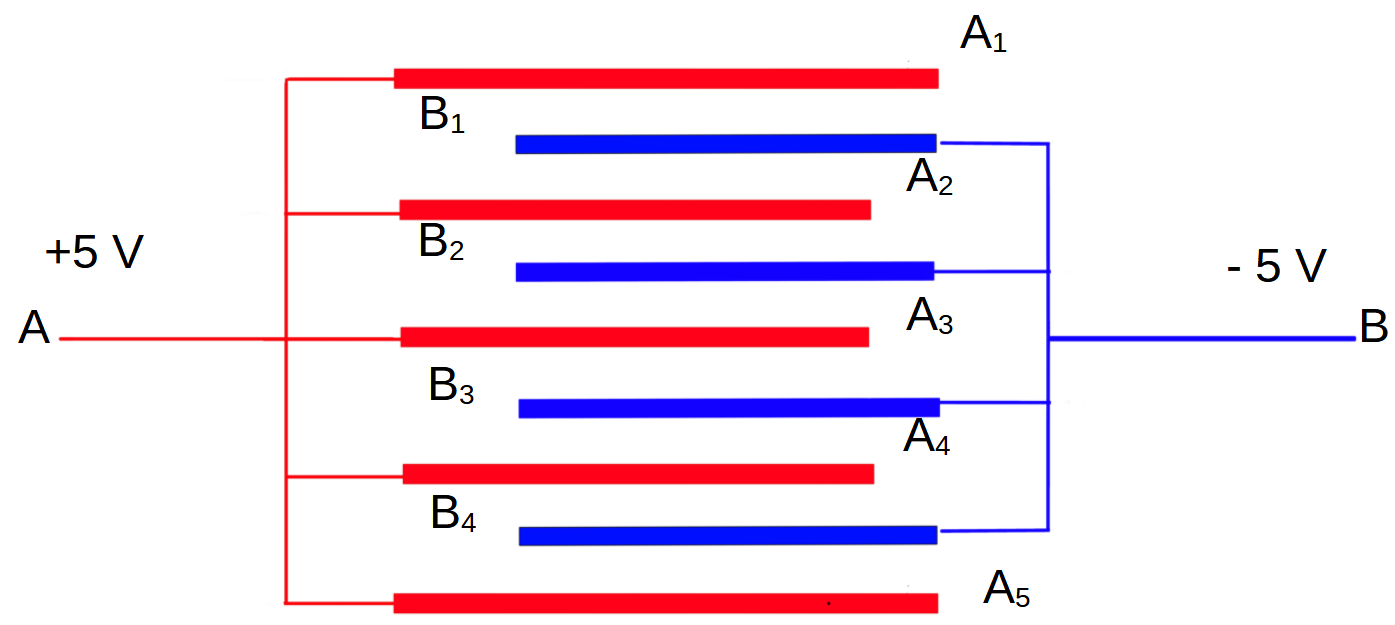
\includegraphics[width=6cm]{insert.png}
				\caption{\small Diagram dipciting the arrangement of plates in a interleaved fashion.}
			\label{fig 1: the capacitor}
			\end{figure}
			After non-dimensionalizing we had following poisson's equation :-
			$$ \frac{\partial^2U'(x',y') }{\partial x^{'2}} + \frac{\partial^2U'(x',y') }{\partial y^{'2}}= -\frac{\rho'(x',y') s^2}{\epsilon_0 \nu} $$
			
		\end{frame}
	\begin{frame}{Problem}
		\begin{equation}
			\rho'(x',y') =  \begin{cases}
				-2\epsilon_0 \times 10^5  & :\text{if} \; (x',y') \in B_i \; \text{where} \; i = 1,2,3,4 \\
				2\epsilon_0 \times 10^5 & :\text{if} \; (x',y') \in A_i \; \text{where} \; i = 2,3,4 \\
				0  & : \; \text{elsewhere}
			\end{cases}
		\end{equation}
		With boundary conditions as -:
		\begin{align}
			& U(0,y) = +5/\nu \quad \ U(4,y) = +5/\nu \\ 
			& U_y(x,0) = 0 \qquad \ U_y(x,4.4) = 0 
		\end{align}
		
		\end{frame}	
	\section{Methodology}
	\begin{frame}[allowframebreaks]{Methodology}
		\subsection{Finite Differences}
		\begin{itemize}
			\item Finite Difference converts PDE into difference equation.
			\item Domain is converted into a mesh of equidistant grid points.
			\item Taylor series is used to approximate the value at  these grid points.
			 \item After using Finite Difference operators we get the following stencil for poisson equation
		\end{itemize}
		\begin{align}
			U_{i,j} = \frac{1}{4} \left[ U_{i+1,j}+ U_{i-1,j} + U_{i,j+1}+ U_{i,j-1} + h^2\frac{\rho'_{i,j} s^2}{\epsilon_0 \nu} \right]
		\end{align}
		\framebreak
		\\
		This stencil can be represented with the help of following diagram
		\begin{figure}
			\centering
			\scalebox{0.56}{
				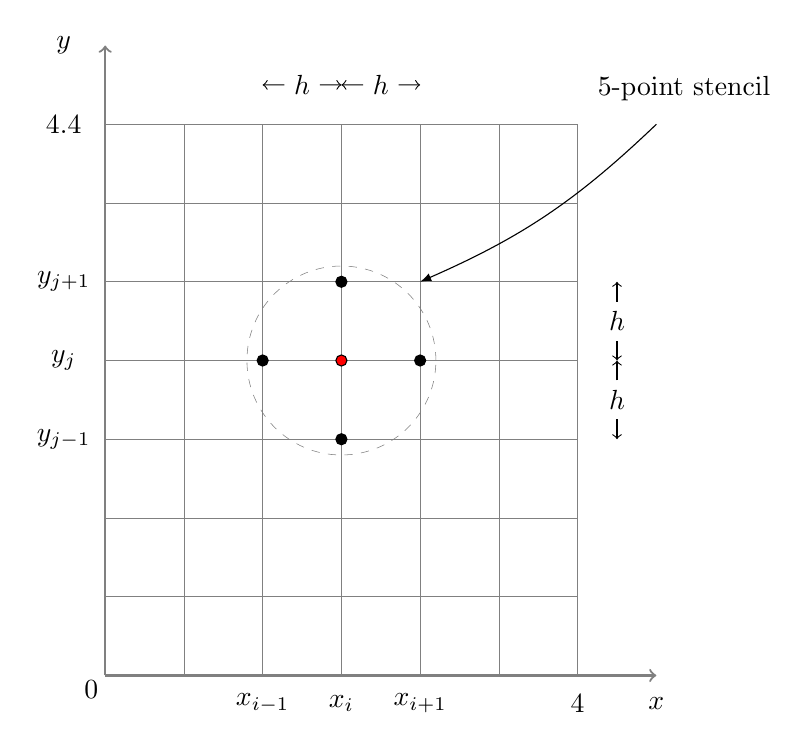
\begin{tikzpicture}
				\coordinate (Y) at (-15pt,8);
				\coordinate (X) at (7,-10pt);
				\draw[step = 1cm,gray, very thin] (0,0) grid (6,7);
				\draw[thick,color=gray,->] (0,0) -- (7,0);
				\draw[thick,color=gray,->] (0,0) -- (0,8);
				\draw (X) node {$x$};
				\draw (Y) node {$y$};
				\draw (X) node[shift={(-4,0)}] {$x_i$};
				\draw (Y) node[shift={(0,-4)}] {$y_j$};
				\draw (X) node[shift={(-5,0)}] {$x_{i-1}$};
				\draw (Y) node[shift={(0,-5)}] {$y_{j-1}$};
				\draw (X) node[shift={(-3,0)}] {$x_{i+1}$};
				\draw (Y) node[shift={(0,-3)}] {$y_{j+1}$};
				\draw (Y) node[shift={(0,-1)}] {$4.4$};
				\draw (X) node[shift={(-1,0)}] {$4$};
				\midlabelline{[shift={(-0.5,3cm + 10pt)}]X}{[shift={(-0.5,4cm +10pt)}]X}{$h$};
				\midlabelline{[shift={(-0.5,4cm +10pt)}]X}{[shift={(-0.5,5cm +10pt)}]X}{$h$};
				\coordinate (Xa) at ([shift={(2cm +15pt,-0.5)}]Y); 
				\coordinate (Xb) at ([shift={(3cm +15pt,-0.5)}]Y); 
				\coordinate (Xc) at ([shift={(4cm +15pt,-0.5)}]Y); 
				\midlabelline{Xa}{Xb}{$h$};
				\midlabelline{Xb}{Xc}{$h$};
				\draw (0,0) node[shift={(-5pt,-5pt)}] {$0$};
				\draw[fill=red] (3,4) circle (2pt) ;
				\draw[fill=black] (4,4) circle (2pt) ;
				\draw[fill=black] (2,4) circle (2pt) ;
				\draw[fill=black] (3,3) circle (2pt) ;
				\draw[fill=black] (3,5) circle (2pt) ;
				\draw[dashed,very thin,color=gray] (3,4) circle (1.2cm) ;
				\draw [latex-] (4cm,5cm) to [bend right=10] (7,7) node[anchor=south,shift={(10pt,5pt)}] {$5$-point stencil};
			\end{tikzpicture}}
		\end{figure}
		\end{frame}	
		\subsection{Truncation Error}
		\begin{frame}{Truncation Error}
			\begin{itemize}
				\item Truncation Error arises due to truncation of Taylor series used for approximating the value of derivative to form a difference equation.
				\item First order derivative can be approximated in three ways-:
					\begin{itemize}
						\item Forward Difference Method
						\item Backward Difference Method
						\item Central Difference Method \\
						\medskip
					\end{itemize}
				
						\begin{center}
							
							\begin{tabular}{ || c| c || } 
								\hline 
								Forward Difference Method &  $ \mcm{O}(\Delta x)$ \\ 
								\hline 
								Backward Difference Method &$ \mcm{O}(\Delta x)$  \\ 
								\hline 
								Central Difference Method &  $ \mcm{O}((\Delta x)^2) $ \\ 
								\hline 
							\end{tabular}
						\end{center}
						\item Above table shows that central order approximation are more accurate than one sided differences.
						\item Second Order derivative is also second order accurate.
				
			\end{itemize}
		\end{frame}
		\subsection{Iterative Methods}
		\begin{frame}[allowframebreaks]{Iterative Method}
			\begin{itemize}

				\item Iterative methods are techniques that exploit the properites of system to solve it implicitly to make computation faster.
				\item We have used following iteratiion schemes-:\\
			
					 \begin{block}{Jacobi Method}
						This method starts with a guess value and with each iteration, it replace guess values with new obtained values from iteration.$$ x^{(n+1)}_{i,j} = S(X^{(n)},P,h,i,j) $$
						\end{block}
					 \begin{block}{Gauss Seidel Method}
						This method uses the obtained value in the same iteration for other unknowns.$$x^{(n+1)}_{i,j} = S(X^{(n+1)},P,h,i,j)$$
						\end{block}
					
					\begin{block}{SOR}
							This method involves a relaxation factor (greater than 1) which is multiplied to values obtained from Gauss Seidel before replacing old values.$$x^{(n+1)}_{i,j} = x^{(n)}_{i,j}+ \omega(S(X^{(n+1)},P,h,i,j)- x^{(n+1)}_{i,j})$$
							
						\end{block}
				
					
					\end{itemize}
				\end{frame}
			\section{Results}
				\subsection{Numerical Results}
				\begin{frame}[allowframebreaks]{Numerical Result}
					We obtained following graphs as solution 
					\begin{figure}
						\centering
						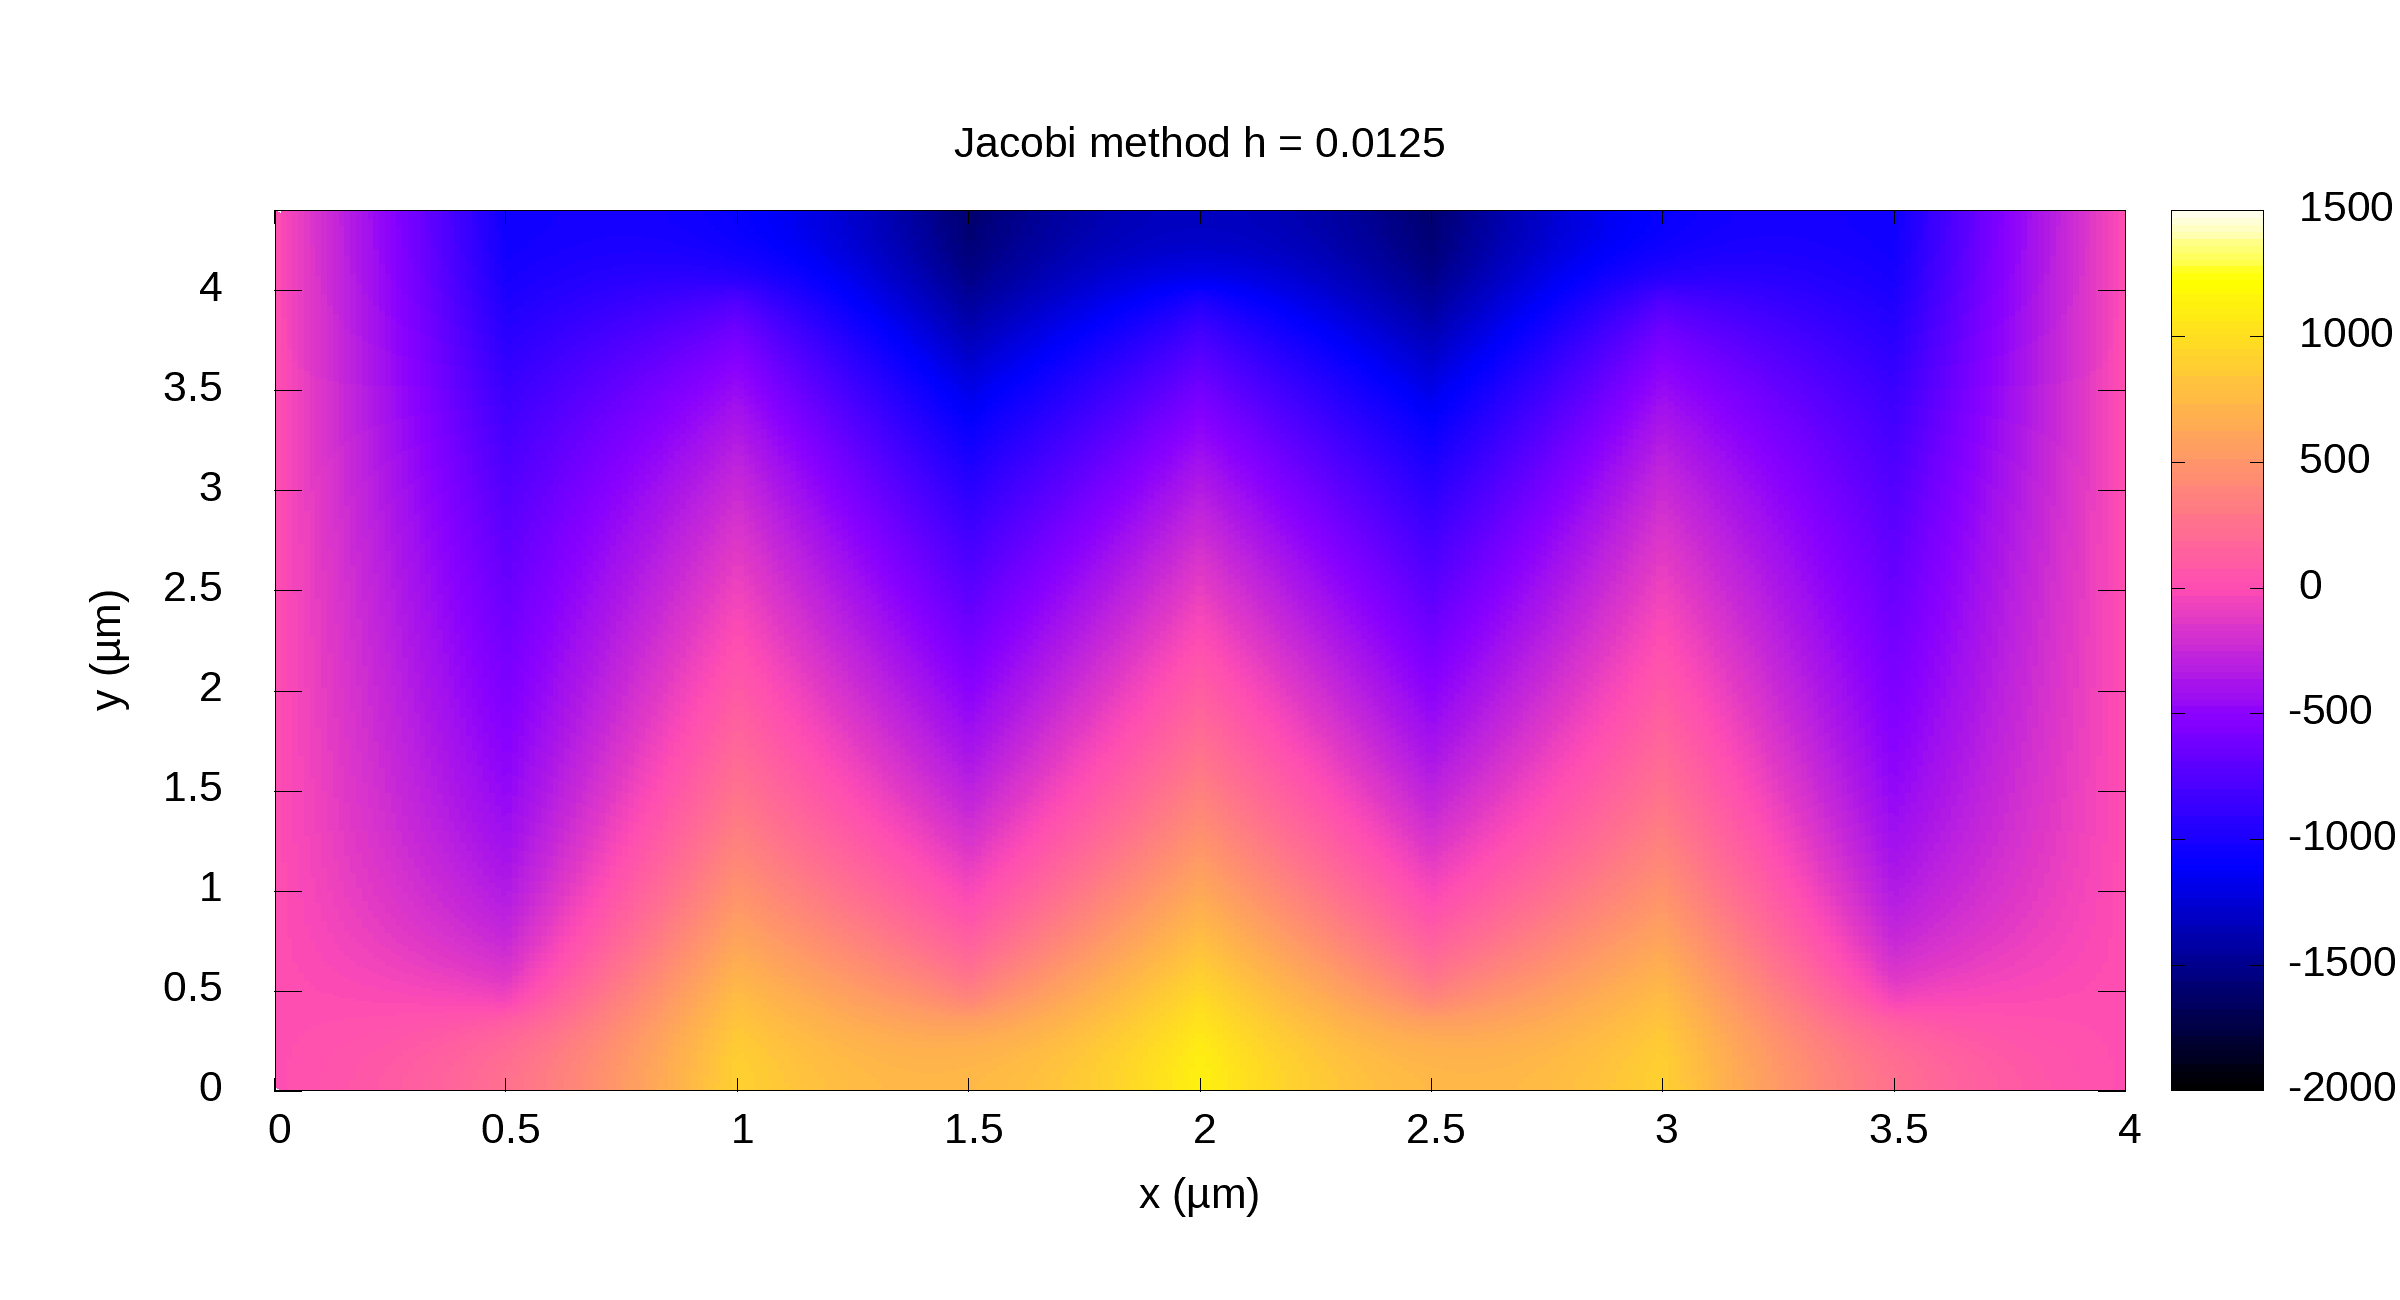
\includegraphics[width=\textwidth]{../report/content/graphs/Jacobi_0125_map.png}
					\end{figure}
					\begin{figure}
						\centering
						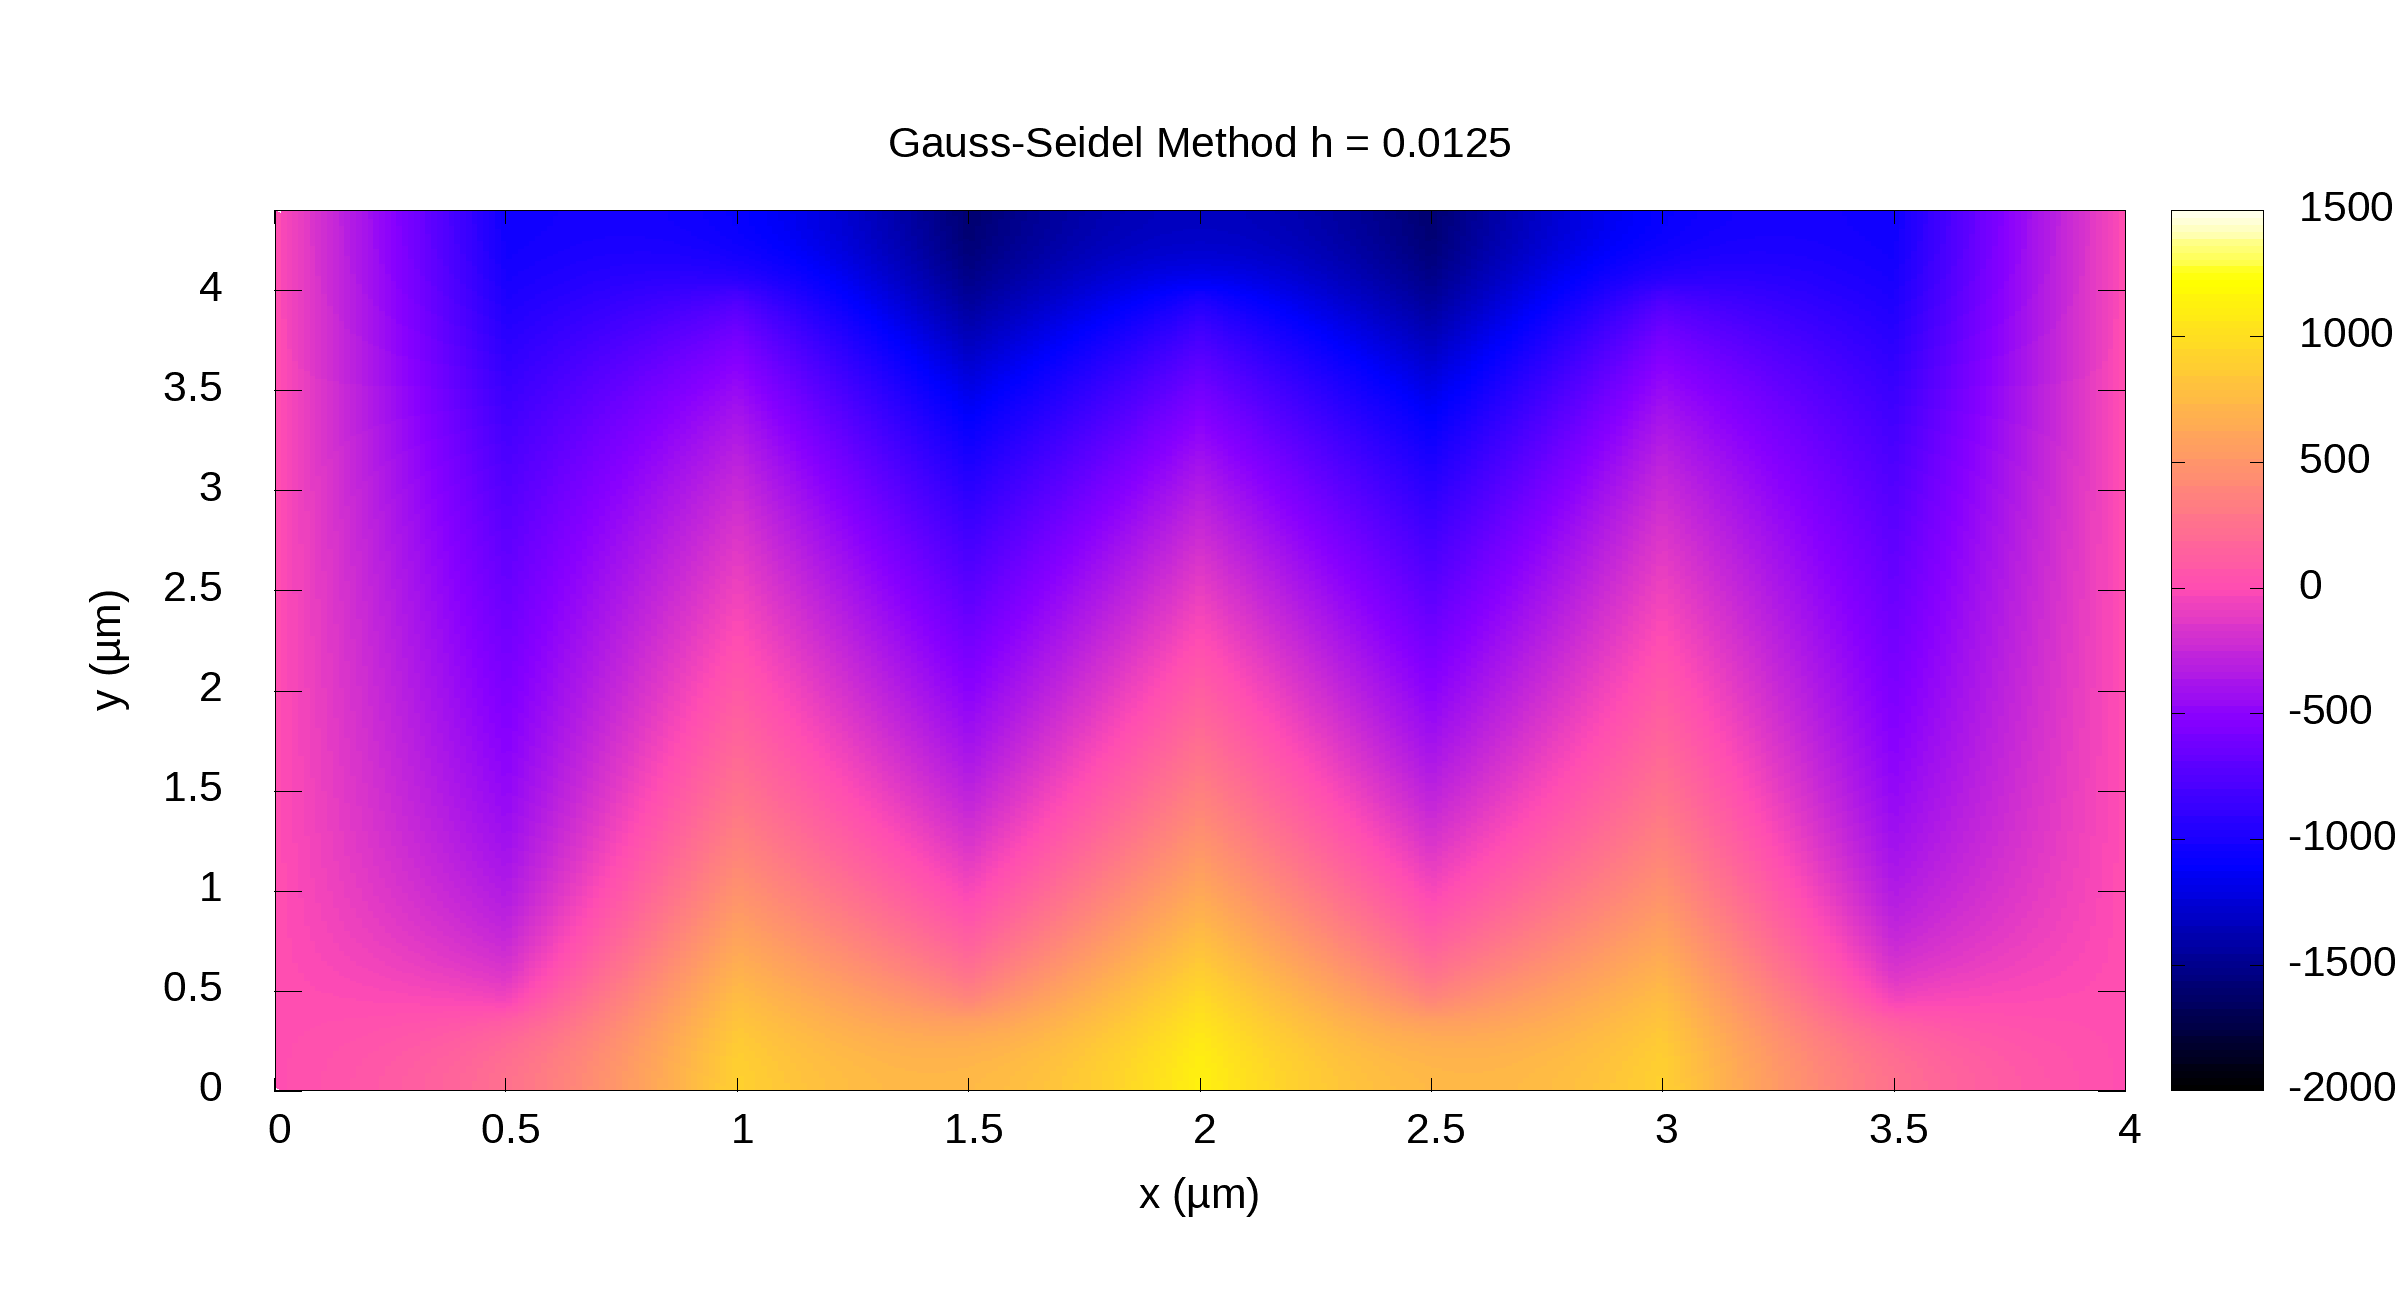
\includegraphics[width=\textwidth]{../report/content/graphs/gauss_map.png}
					\end{figure}
					\begin{figure}
						\centering
						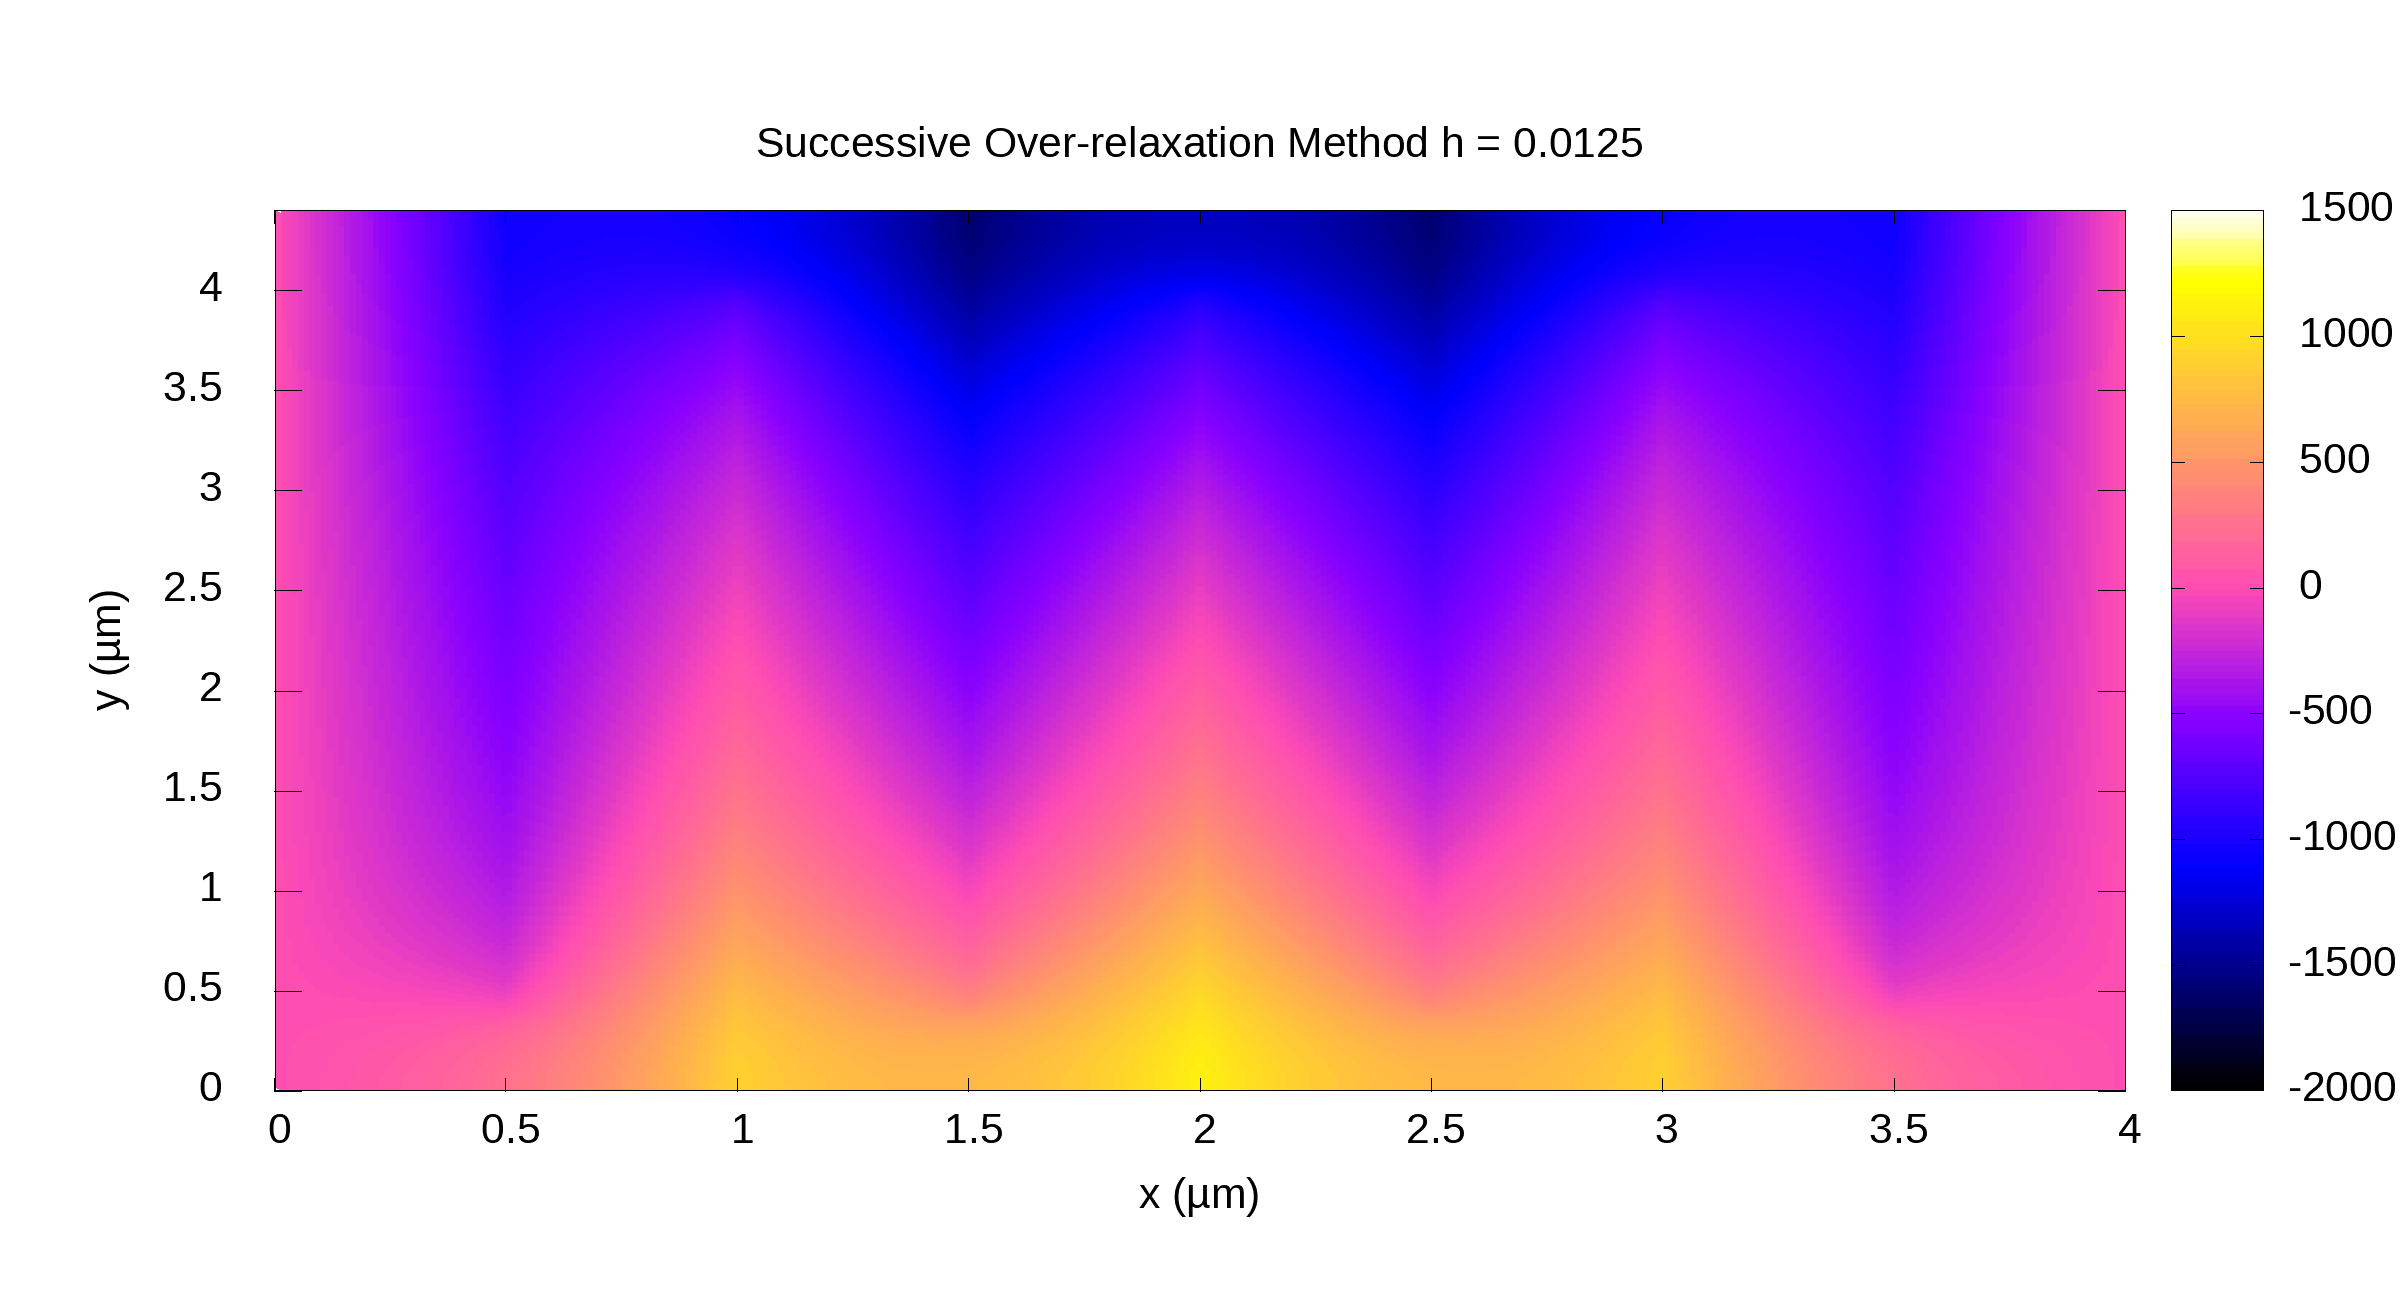
\includegraphics[width=\textwidth]{../report/content/graphs/sor_map.png}
					\end{figure}
					\subsection{About relaxation factor $\omega$}
					\begin{figure}
						\centering
						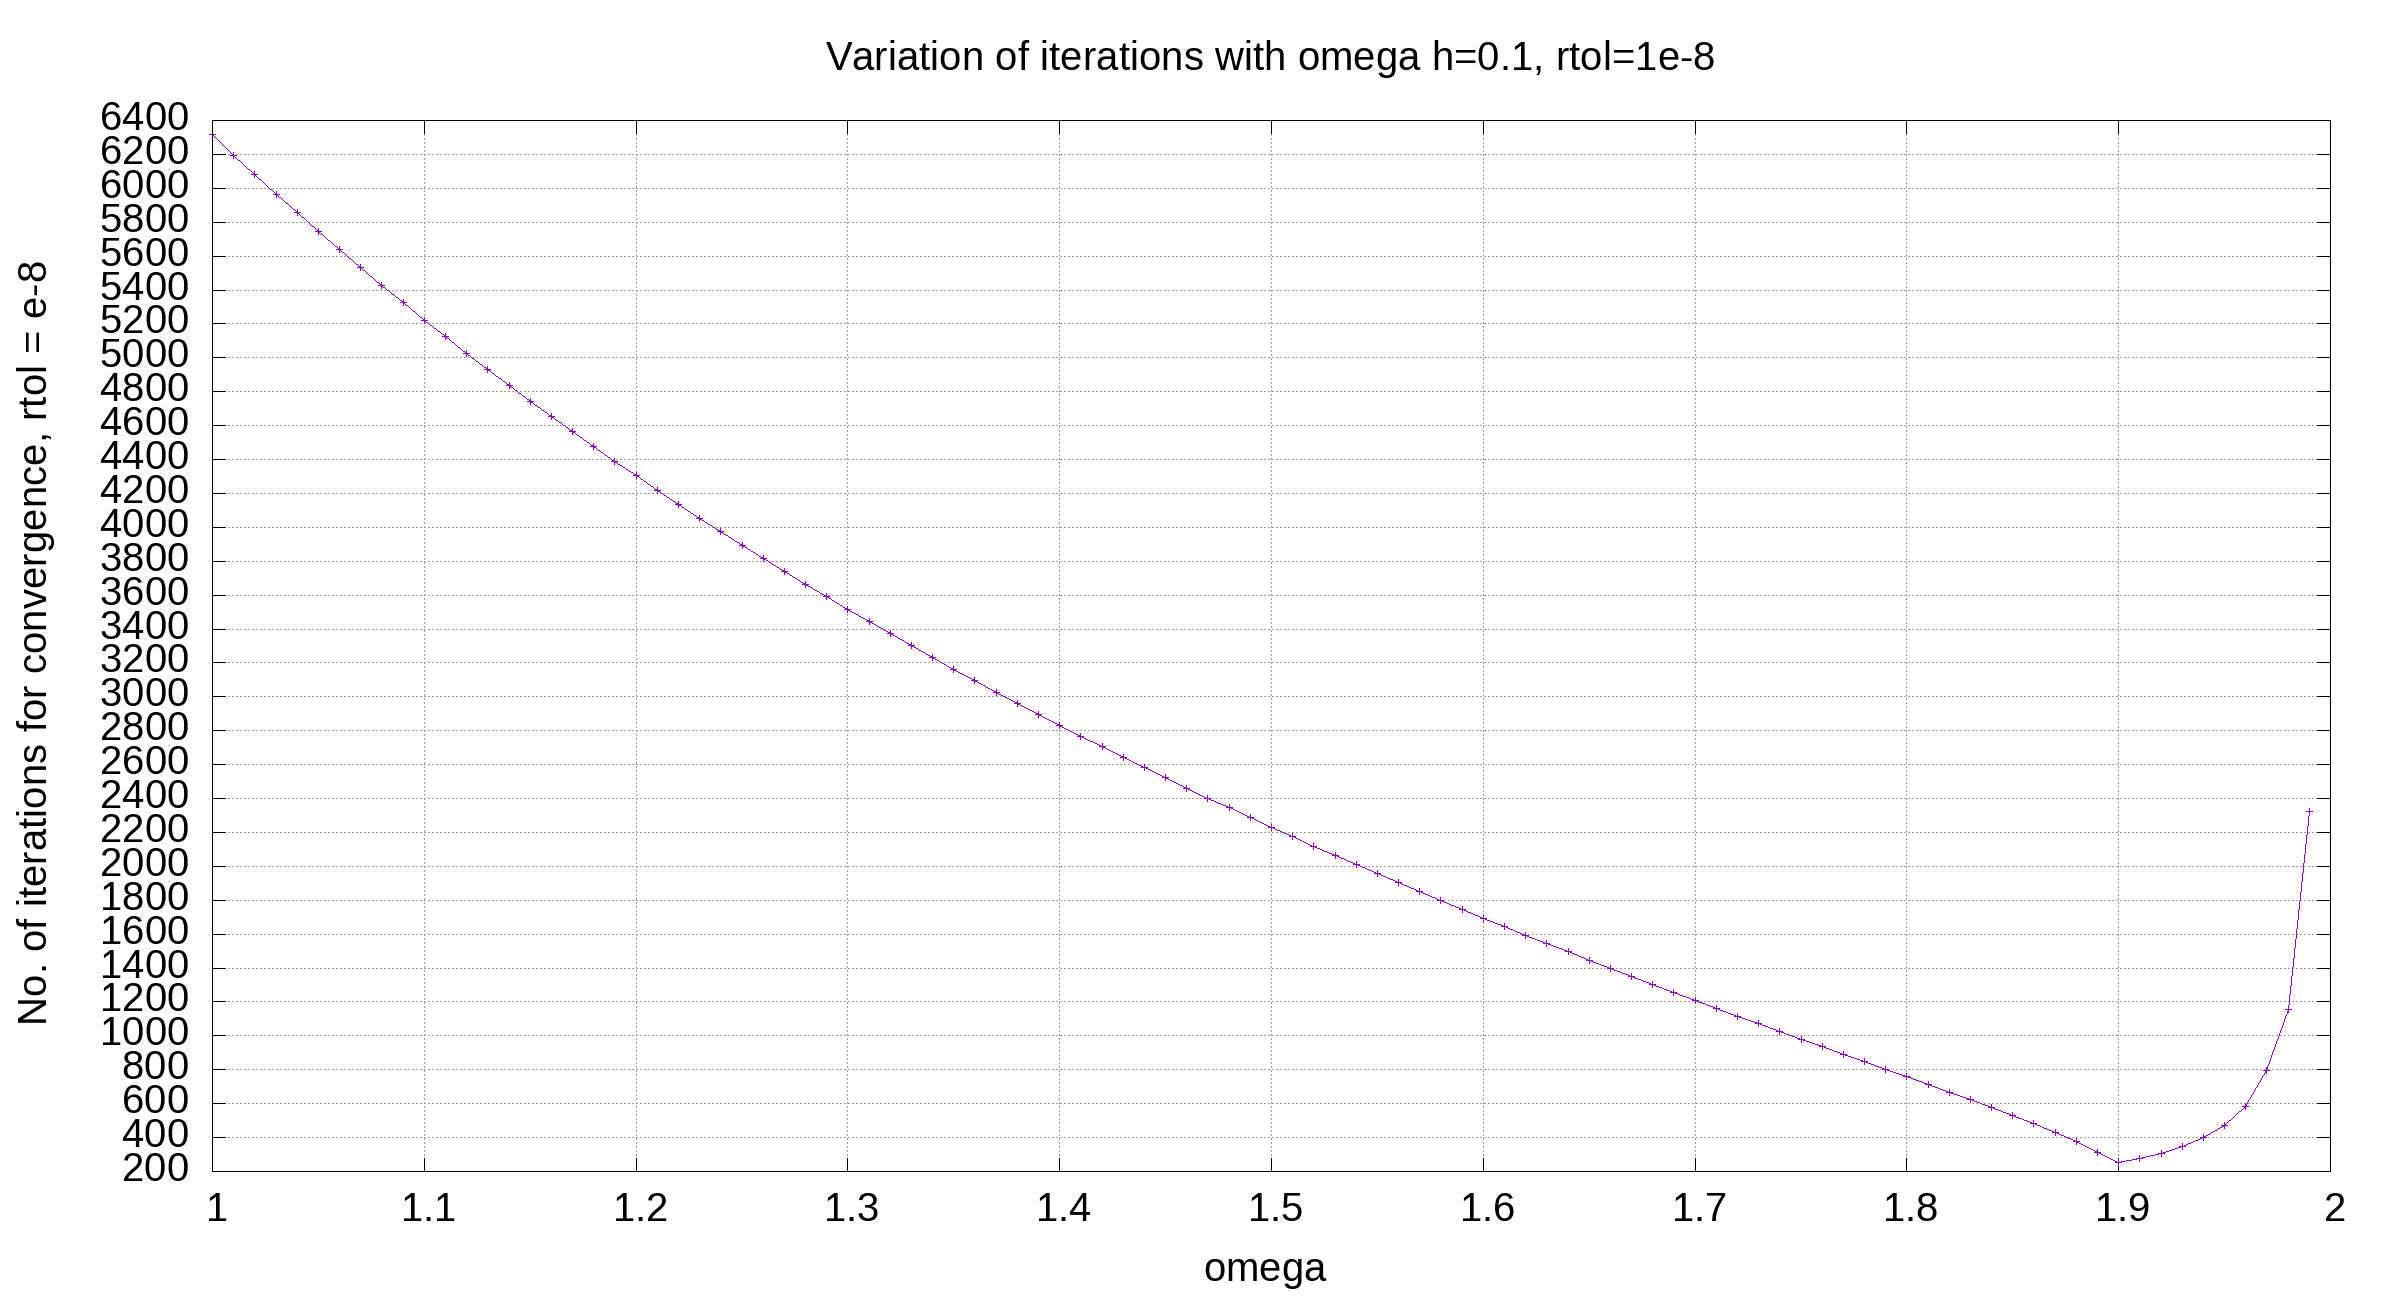
\includegraphics[width=\textwidth]{../report/content/graphs/omega.png}
					\end{figure}
					
				\end{frame}
				\section{Conclusion}
					\begin{frame}{Conclusion}
						\begin{block}{Result}
							\begin{itemize}
								\item After computing thte problem of interleaved capacitor from three different iterative schemes, we have arrived at the conclusion that SOR is the fastest among three.
							\end{itemize}
							\end{block}
						\begin{block}{Experiences}
							\begin{itemize}
								\item We gained better intuition and it has helped us to gain a better grasp on the concept of electrostatic potential.
								\item We learnt the method of finite differences which lies at the core of many computational methods for differential equation.
								\item This project has also introduced us to delight of finding out new things, as most of things we did in this project were completely new to us.
							\end{itemize}
						\end{block}

					\end{frame}
				\begin{frame}[allowframebreaks]{References}
					\nocite{*}
					\printbibliography[heading=none]
				\end{frame}
\end{document}

